% !TEX root = ../ClassicThesis_DEIB.tex

\chapter{Experimental results} \label{chap:experimentalResults}

On the field sessions were a crucial point in the validation of \ac{GRAPE} system, for two main reasons:
\begin{enumerate}
	
	\item Robotics is a field that, by definition, requires interaction with the physical world, both the components of the robot itself, and the environment. Thus, simulation could strongly speed up the the development in certain phases, but the creation of a robotic system cannot opt out of experimental sessions. This consideration is especially true in agricultural robotics field, because a simulated environment or a laboratory environment are extremely likely to be too different from the actual robot environment to be significant.

	\item As explained in Section \ref{sec:grapeProjectDescription}, the research team included members from both Politecnico di Milano and Eurecat, that are located in two different countries. Even if this should not have been a big problem, the division of labor created significant inefficiencies because:
	\begin{itemize}
		\item even if the sensor fusion and navigation parts were assigned to Politecnico, the Husky \ac{UGV} was property of Eurecat, so it was in Barcellona
		\item even if the analysis of the vine scan in order to detect the most suitable deployment point was in charge of Eurecat, the arm was property of Politecnico so it was in Milano.
	\end{itemize}
	This problem was mitigated by the logging tool of \ac{ROS} (\textit{rosbag} package we mentioned in Section \ref{sec:robotOperatingSystem}), that demonstrated its potential in such a situation: \textit{bags} recorded during (non-autonomous) navigation sessions of the Husky were very useful to test the sensor fusion system, while \textit{bags} of the laser scans sensed during execution of the scan motion in front of the mockup vine (see Figure \ref{fig:mockupPlant}), owned by Politecnico team. However, the usage of \textit{bags} in our context showed two main weaknesses, the first of which is is specific of our context, while the second is intrinsic to the use of recorded data:
\begin{itemize}
	\item autonomous navigation algorithms cannot be tested by means of recorded data \textit{bags} because, during an autonomous navigation session, the data that are sensed while using a specific navigation algorithm depend on the choices of the algorithm itself; the same reasoning does not apply to neither sensor fusion nor point cloud analysis tasks.
	For this reason, the only way to test a navigation algorithm except for \textit{on-the-field} experiments is via simulation by means of a physical simulator. Some effort were spent in this direction before the beginning of this thesis work (see Section \ref{sec:thesisInGrape}), but very few \textit{on-the-field} tests have been enough to show that the simulated environment was way too different from the real one for the test to be significant.
	\item validation of algorithms by means of recorded data significantly increases the risk of overfitting \textit{i.e.} adapting the model only to perform well with the data in the (few) \textit{bags} at disposal, and not new new data coming, for example, from an \textit{on-the-field} experiment. The best ways to decrease the probability of overfitting are:
	\begin{itemize}
		\item use as many bags as possible in testing and validation phase
		\item test in the real environment as often as you can. Remember, however, that sometimes overfitting can occur also in real environment, in less obvious way. For example, the ROAMFREE configuration executed in Mas Llunes during the first integration week was absolutely ineffective when applied in Casciano Terme vineyard, because it fitted too tightly the features of Mas Llunes vineyard thus it didn't represent a general solution.
	\end{itemize}
\end{itemize}

\end{enumerate}

\section{Sensor fusion}

\begin{figure}
	\centering
	\subfloat[]{%
		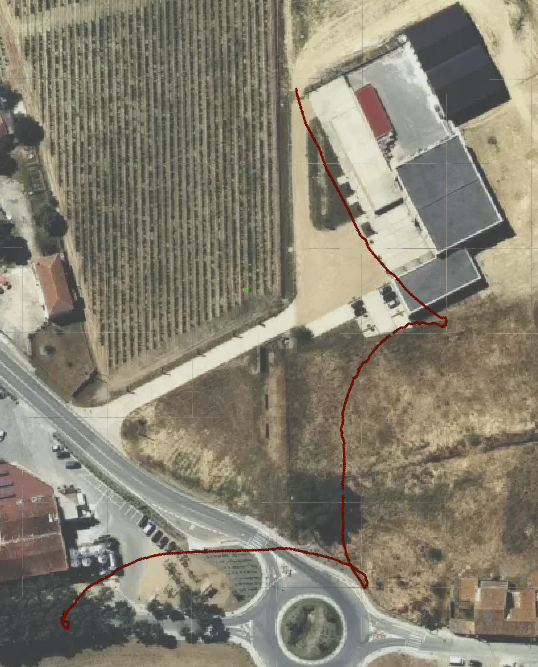
\includegraphics[width=0.65\textwidth]{Images/experimental_data/wheels_3.png}
		\label{fig:wheelsOdometryRes}} \\
	\subfloat[]{%
		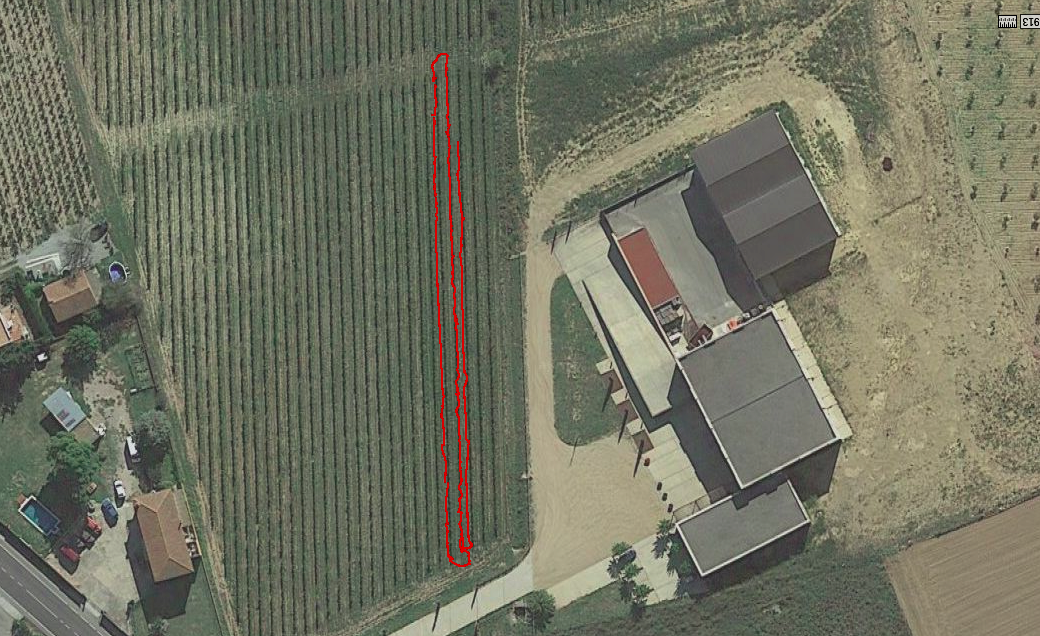
\includegraphics[width=0.65\textwidth]{Images/experimental_data/gpsRaw_dark.png}
		\label{fig:gpsRawRes}}
	\caption{\textit{Pose estimation in time using raw wheels odometry (Figure \ref{fig:wheelsOdometryRes}), and using GPS (Figure \ref{fig:gpsRawRes}).}}
	\label{fig:sensorFusionInputs}
\end{figure}

\begin{figure}
	\centering
	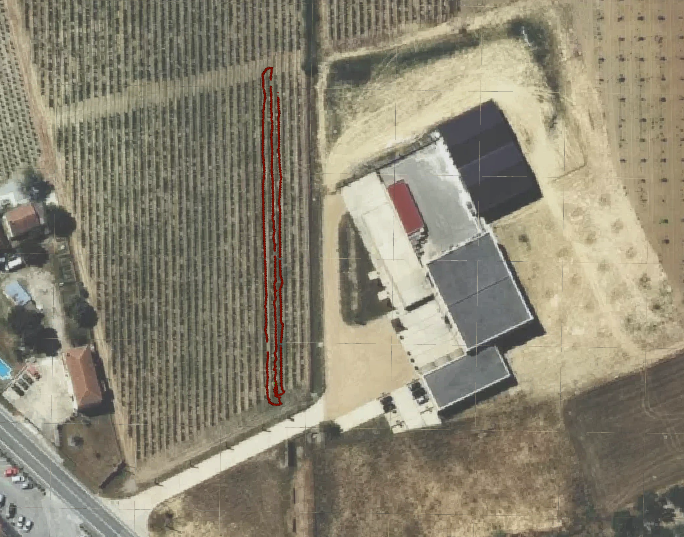
\includegraphics[width=0.75\textwidth]{Images/experimental_data/rob_loc_result.png}
	\caption{\textit{The odometry estimated by Robot Localization sensor fusion framework, fusing (among others) the pose estimated by the wheels (see Figure \ref{fig:wheelsOdometryRes}) and by the GPS (see Figure \ref{fig:gpsRawRes})}}
	\label{fig:wheelsOdometryRes}
\end{figure}

\section{Navigation}

\begin{figure}
	\begin{minipage}[c]{.5\textwidth}
	\centering
	\subfloat[]{%
		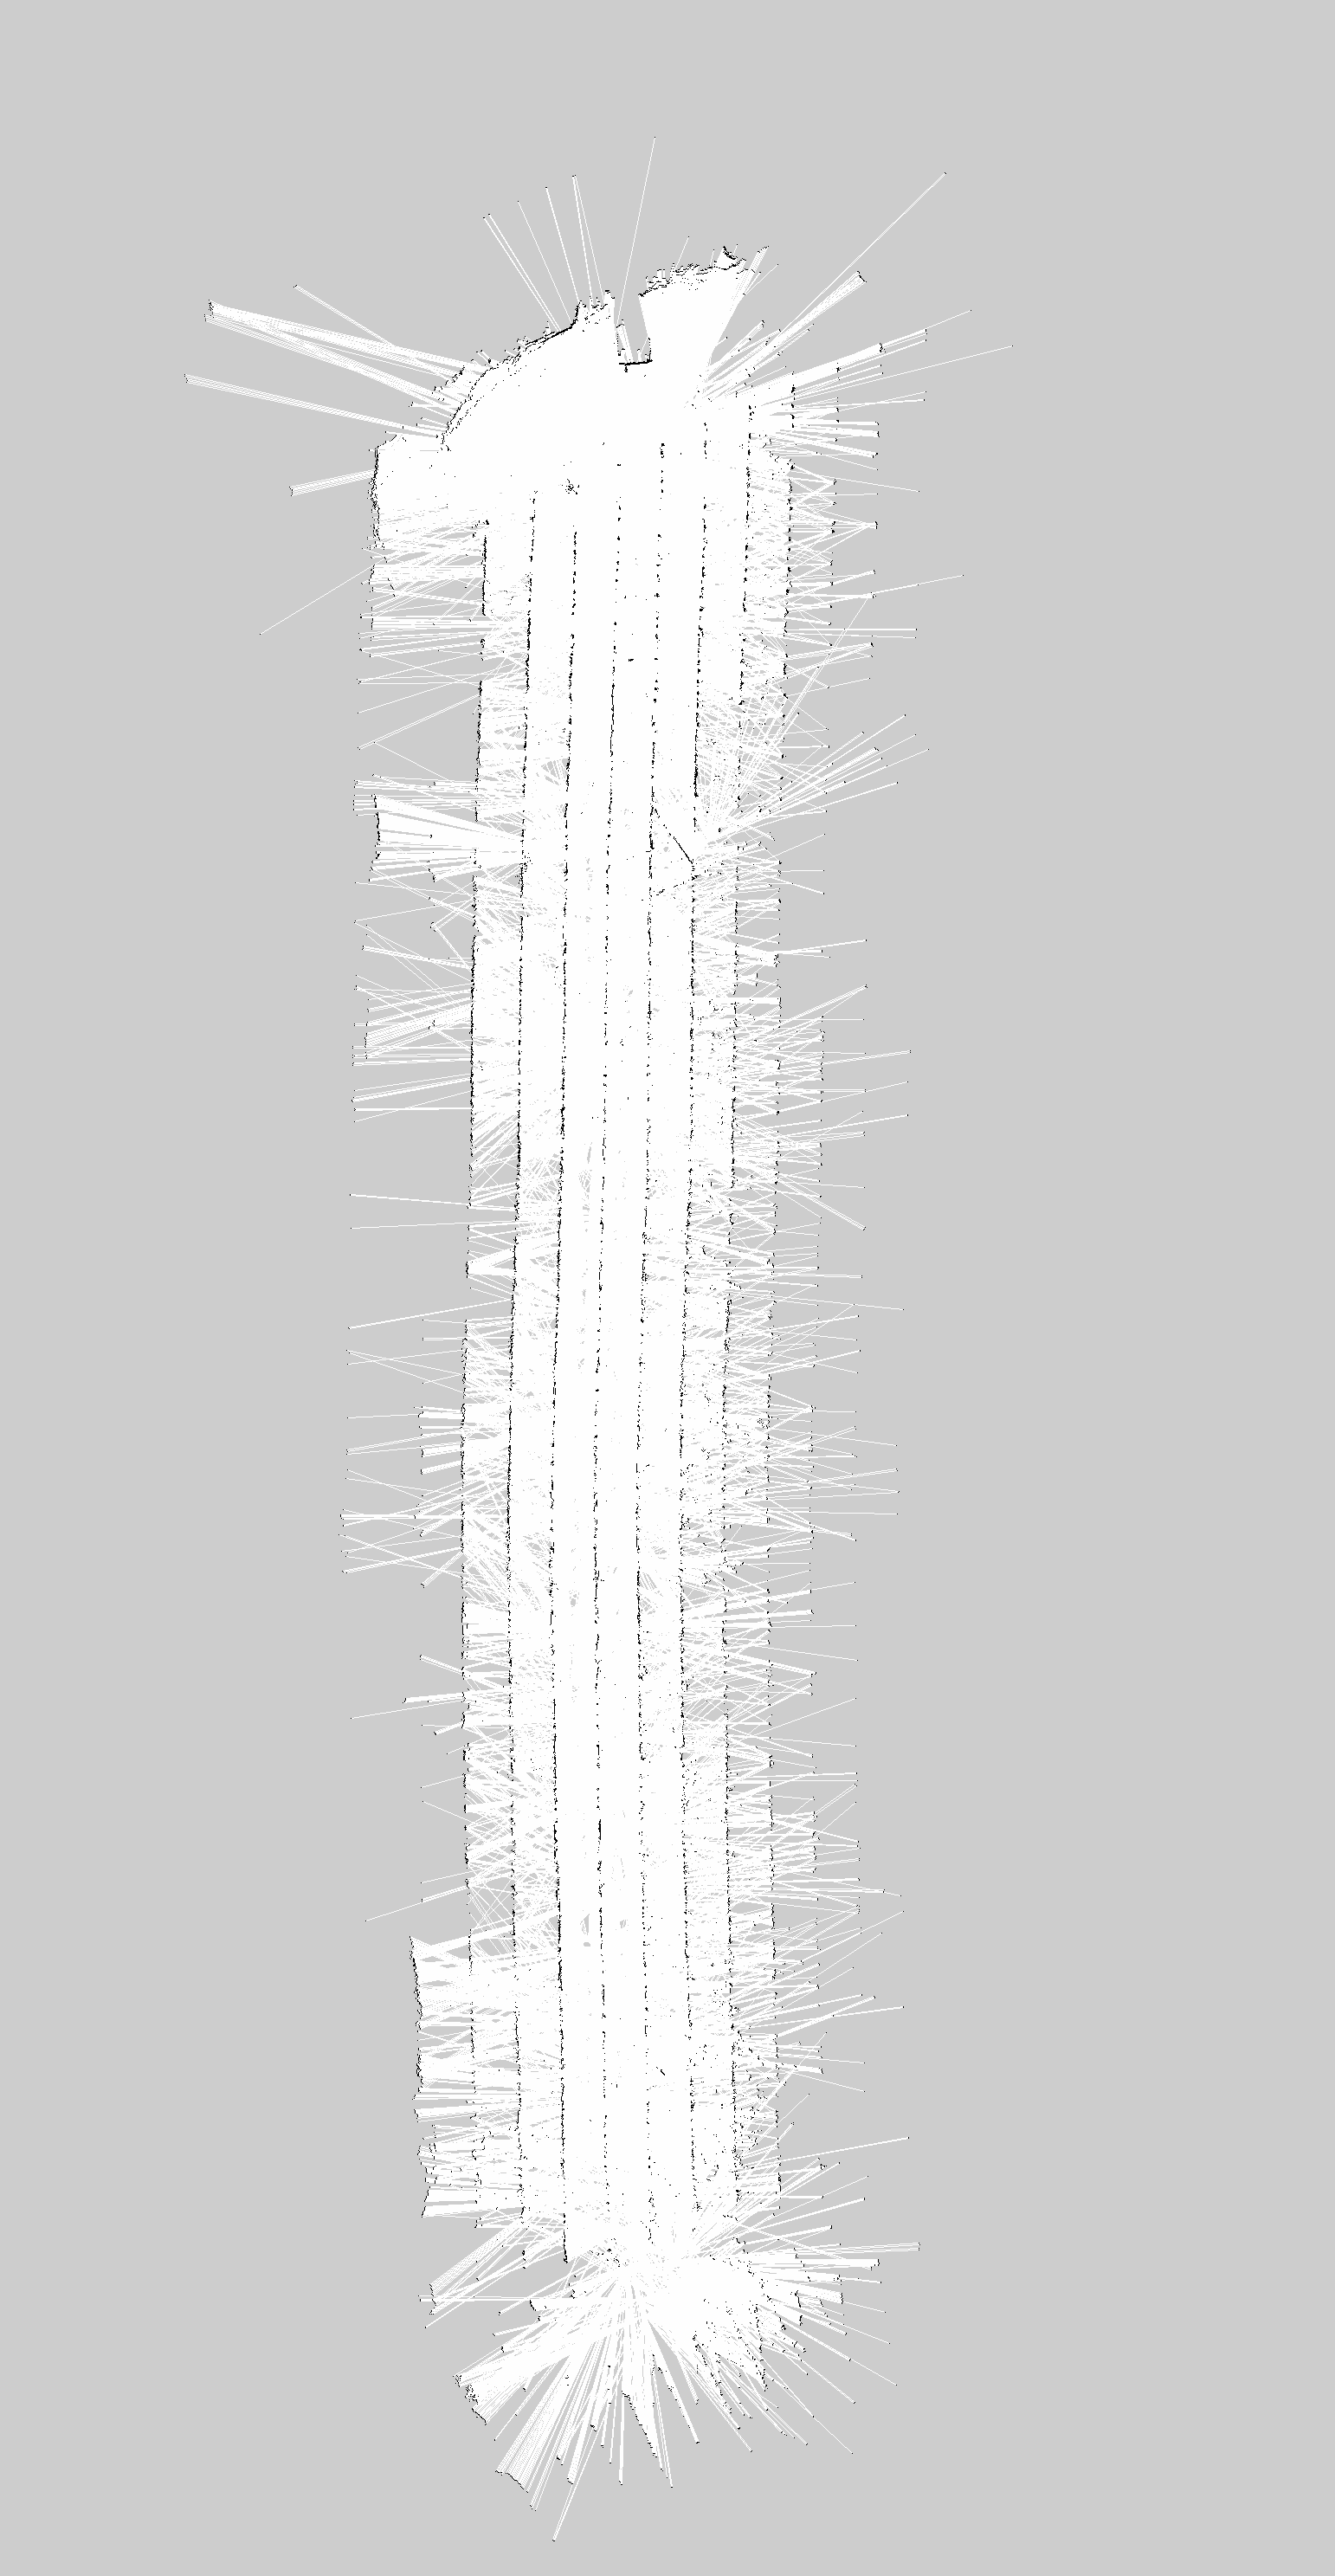
\includegraphics[width=0.7\textwidth]{Images/experimental_data/masLlunes_map.png}
		\label{fig:mapResult_masLlunes}}
	\end{minipage}
	\begin{minipage}[c]{.5\textwidth}
	\subfloat[]{%
		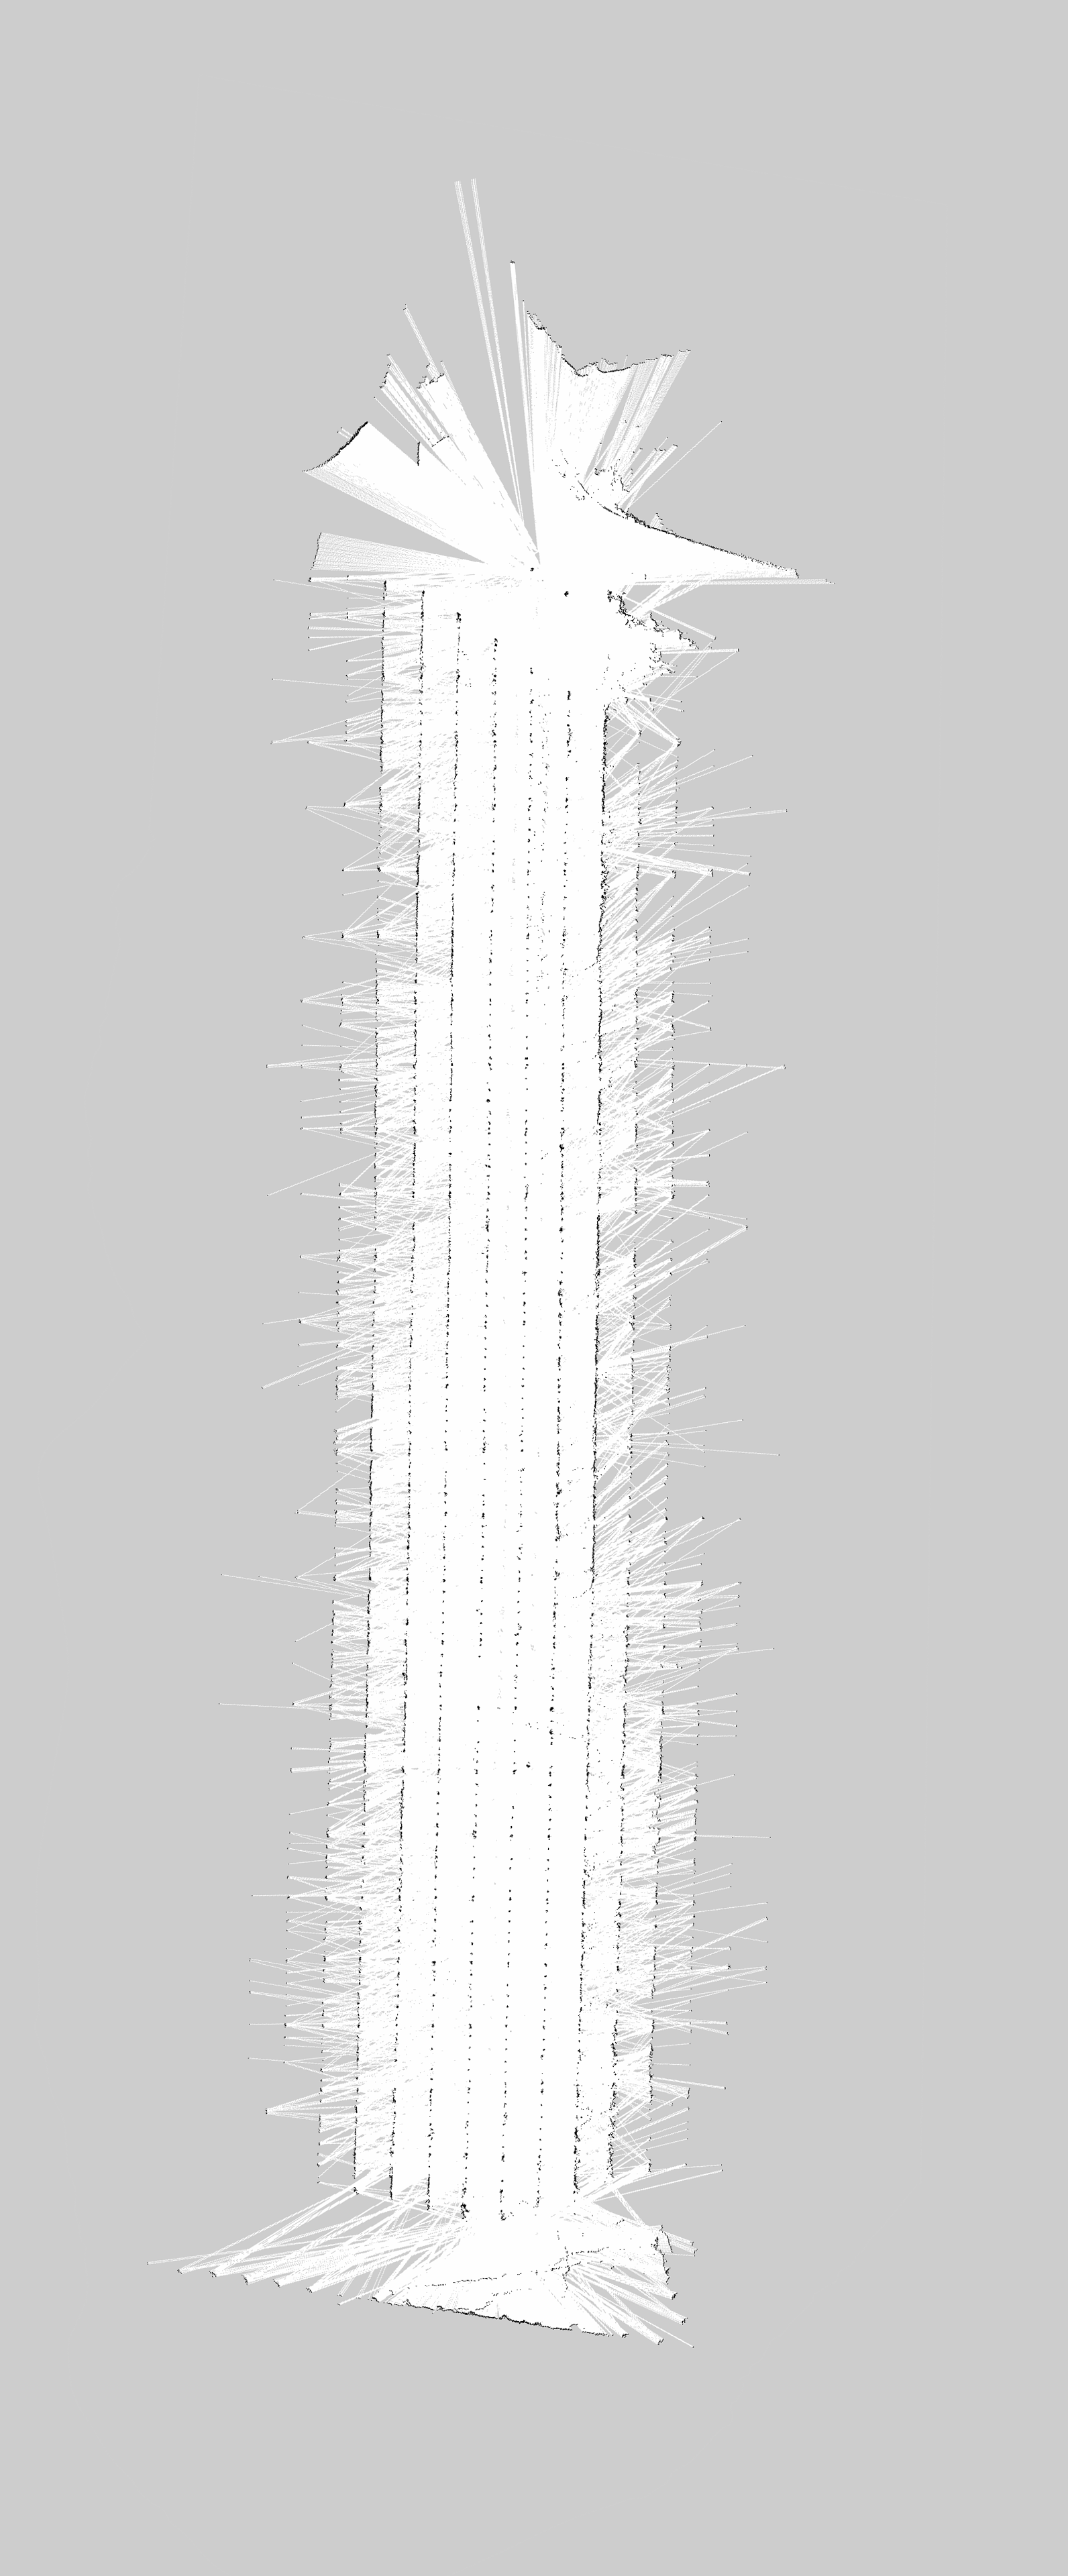
\includegraphics[width=0.65\textwidth]{Images/experimental_data/toscana_map.png}
		\label{fig:mapResult_toscana}}
	\end{minipage}
	\caption{\textit{Output of mapping phase, using Gmapping as \ac{SLAM} algorithm and Robot Localization as sensor fusion framework.}}
	\label{fig:sensorFusionInputs}
\end{figure}


\begin{figure}
	\centering
	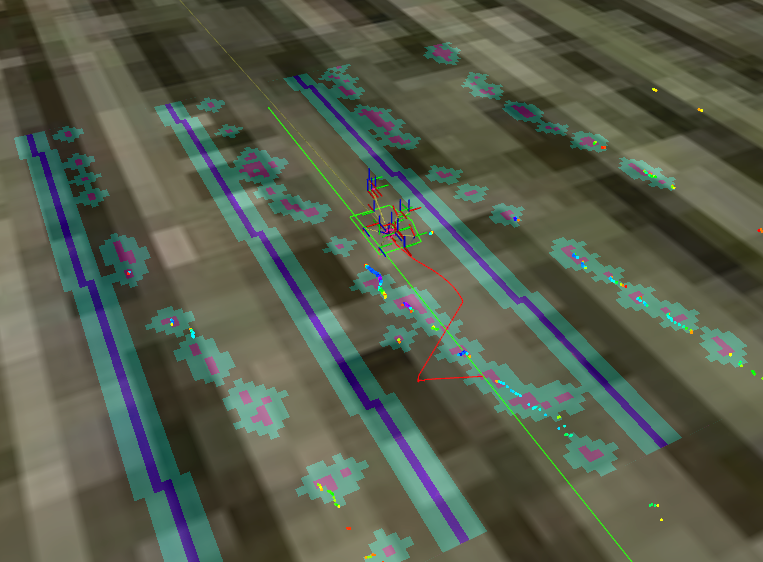
\includegraphics[width=0.8\textwidth]{Images/experimental_data/navigation2_gimped.png}
	\caption{\textit{Visualization through RViZ of the Husky performing autonomous navigation, with the local costmap overlaid to the satellite images of Mas Llunes vineyard. You can see the global (green line) and local (red line) navigation plans, the} tf \textit{tree of the robot and the Husky footprint used by Move Base for the interaction with the costmap.}}
	\label{fig:result_navigation}
\end{figure}


\section{Manipulation}


\begin{figure}
	\centering
	\subfloat[]{%
		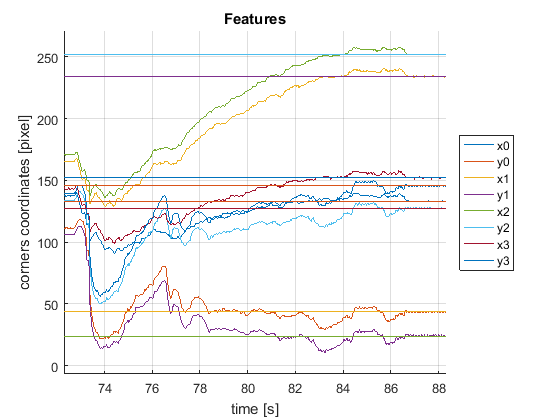
\includegraphics[width=0.65\textwidth]{Images/experimental_data/deployment_nail_features.png}
		\label{fig:deploymentNailFeatures}}
	\subfloat[]{%
		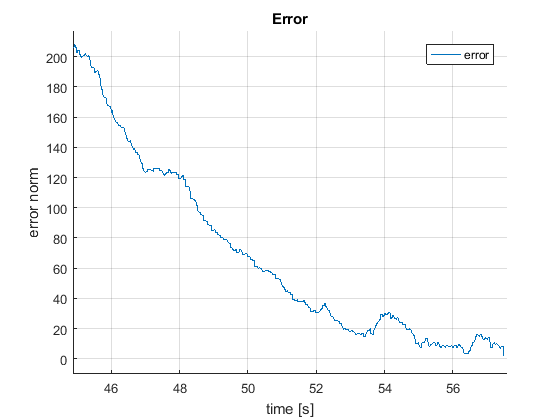
\includegraphics[width=0.65\textwidth]{Images/experimental_data/deployment_nail_error.png}
		\label{fig:deploymentNailError}}
	\caption{\textit{Evolution in time of the image coordinates of the corners of the tracked marker (see Figure \ref{fig:deploymentNailFeatures}) during visual servoing driven deployment of a dispenser on a nail. In Figure \ref{fig:deploymentNailError}, the evolution in time of the module of the error on the tracked features.}}
	\label{fig:deploymentNailResult}
\end{figure}

\begin{figure}
	\centering
	\subfloat[]{%
		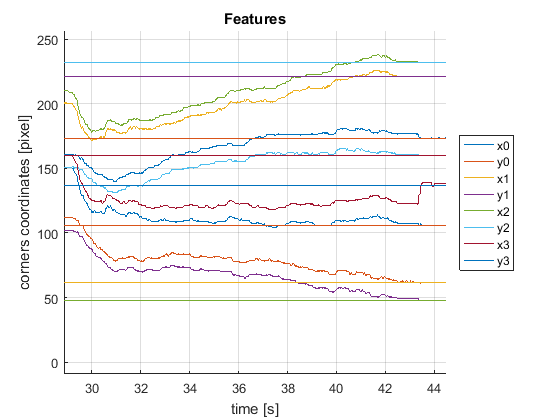
\includegraphics[width=0.65\textwidth]{Images/experimental_data/grasping_low_features.png}
		\label{fig:graspingFeatures}}
	\subfloat[]{%
		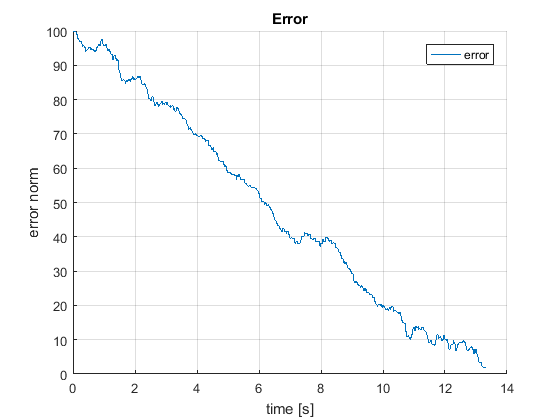
\includegraphics[width=0.65\textwidth]{Images/experimental_data/grasping_low_error.png}
		\label{fig:graspingError}}
	\caption{\textit{Evolution in time of the image coordinates of the corners of the tracked marker (Figure \ref{fig:graspingFeatures}) during visual servoing driven grasping of the dispenser from the feeder. In Figure \ref{fig:graspingError}, the evolution in time of the module of the error on the tracked features,}}
	\label{fig:graspingLowResult}
\end{figure}



\begin{figure}
	\centering
	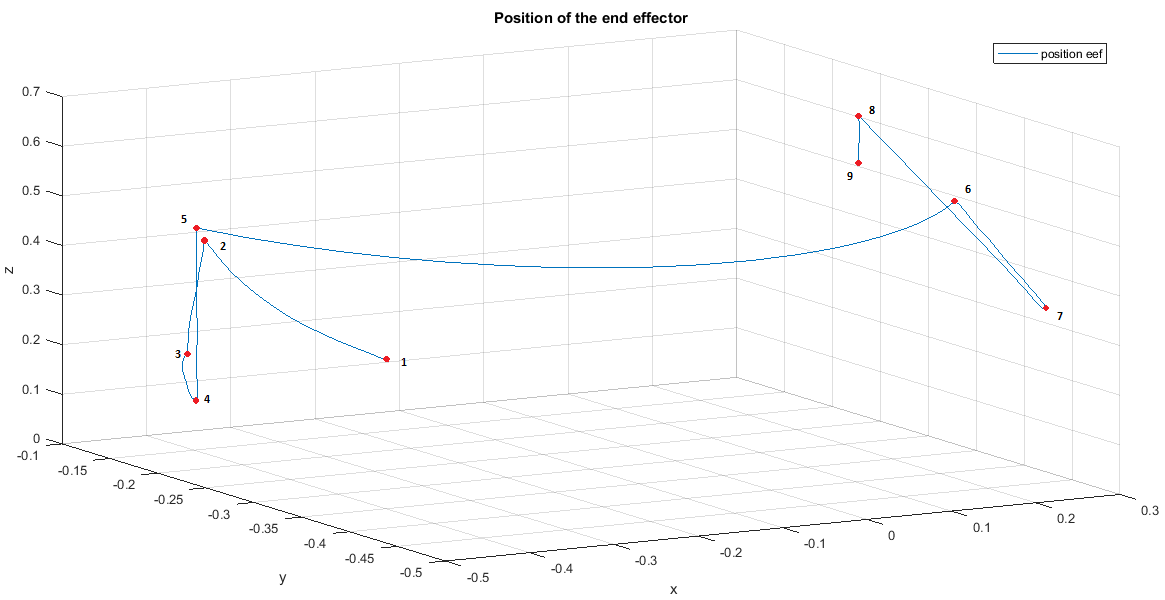
\includegraphics[width=0.9\textwidth]{Images/experimental_data/depl_moveit_endeffector.png}
	\caption{\textit{Evolution of the 3D $(x,y,z)$ position of the end effector of the Jaco$^2$ during dispenser deployment using MoveIt!}}
	\label{fig:deplMoveitEndEffect}
\end{figure}

\begin{figure}
	\centering
	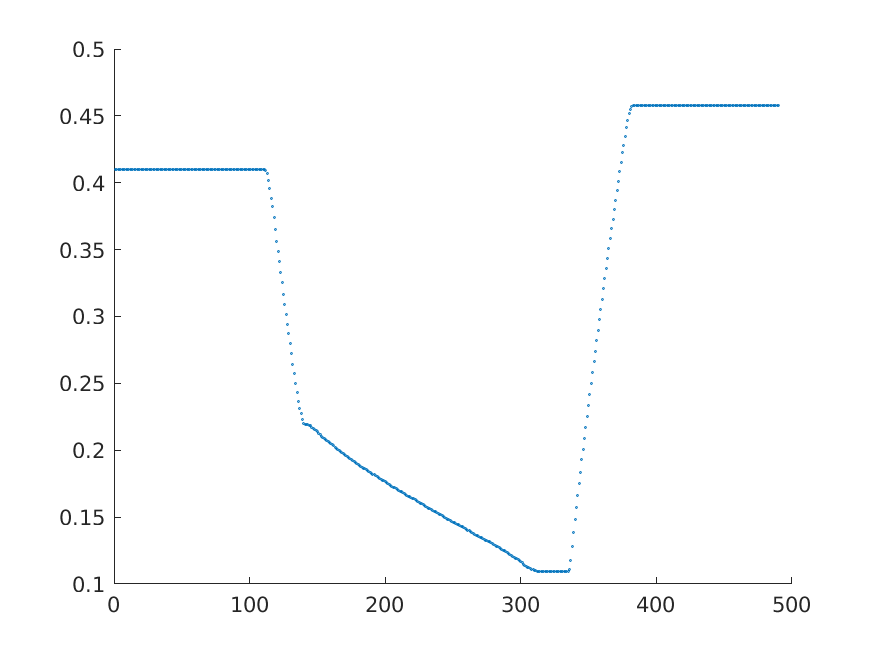
\includegraphics[width=0.9\textwidth]{Images/experimental_data/grasping_z.png}
	\caption{\textit{Evolution of the $z$ coordinate of the end effector, during visual servo driven grasping of the dispenser from the feeder.}}
	\label{fig:graspingZ}
\end{figure}






